% sPDMX — ICASSP proceedings draft
% Uses: spconf.sty, IEEEbib.bst
% --------------------------------------------------------------------------
\documentclass{article}
\usepackage{spconf,amsmath,graphicx,hyperref,booktabs,multirow}

\title{sPDMX: Large-Scale Stem Audio from Symbolic Music via Listening-Tuned Synthesis}

\name{Phillip Long, Eduardo Escoto, Julian McAuley, Zachary Novack}
\address{University of California, San Diego}

\begin{document}
%\ninept
%
\maketitle
%
\begin{abstract}
Large multitrack audio datasets enable training of generative and separation models, but recorded stems are scarce and synthetically rendered MIDI often sounds unrealistic.
We present \textbf{sPDMX}, a pipeline that converts the public-domain symbolic corpus PDMX into multi-stem audio with controllable synthesis quality.
Starting from FluidSynth renders, we introduce Slakh-style per-category soundfont variety, optional neural DDSP synthesis, and Stable Audio~3 audio-to-audio ``realify.''
Per-category rendering and realify settings are locked via blinded tuning listening tests.
We then compare eight factorial ablation conditions in a dual-scale listening study (content adherence and realism) and select a production recipe for the full dataset.
Finally, we train Stable Audio Open from scratch on Slakh2100 versus sPDMX and evaluate listener preference on held-out generations.
% Results placeholders filled after studies complete.
\end{abstract}
%
\begin{keywords}
Symbolic music, stem synthesis, listening tests, generative audio, dataset construction
\end{keywords}
%
\section{Introduction}
\label{sec:intro}

Multitrack stem audio is central to music source separation, accompaniment generation, and controllable audio models.
Recorded corpora such as MUSDB18~\cite{rafii2019musdb18} and MedleyDB~\cite{bittner2014medleydb} offer high realism but limited scale and genre coverage.
Synthesized alternatives such as Slakh2100~\cite{manilow2019cutting} expand volume via professional sample libraries, yet remain smaller than modern symbolic collections and are tied to closed virtual instruments.

PDMX~\cite{long2024pdmx,xu2024generating} provides a large public-domain MusicXML/MIDI resource, but naive soundfont rendering yields dry, recognizably synthetic stems.
After correcting mismatched GM program IDs from track names, PDMX stem mass concentrates in acoustic piano, choir/voice, drums, and common orchestral winds, brass, and strings (Fig.~\ref{fig:gm_programs}).
The gap we address is a \emph{scalable, open, listening-tuned} path from symbolic scores to stem-level audio suitable for training generative models, with realify effort allocated where the corpus is densest.

We introduce \textbf{sPDMX}: a synthesis pipeline and dataset construction protocol with four contributions.
(i)~A MIDI-to-stems pipeline combining GM register correction, FluidSynth~\cite{fluidsynth} rendering, Slakh-inspired per-category soundfont shortlists and light FX, optional DDSP neural synthesis~\cite{engel2020ddsp,wu2022midi,renault2022diffpiano,renault2023ddsp_piano}, and Stable Audio~3 (SA3)~\cite{evans2026stable} realify.
(ii)~Per-instrument-category tuning of Slakh patches and SA3 presets via blinded dual-scale listening, prioritized for piano, voice, and orchestral families that dominate PDMX.
(iii)~A formal $4{\times}2$ ablation listening study (render family $\times$ realify) that selects the production recipe.
(iv)~A downstream experiment training Stable Audio Open (SAO)~\cite{evans2024stable} on Slakh2100 versus sPDMX, with preference listening on model outputs.

\begin{figure}[t]
  \centering
  \centerline{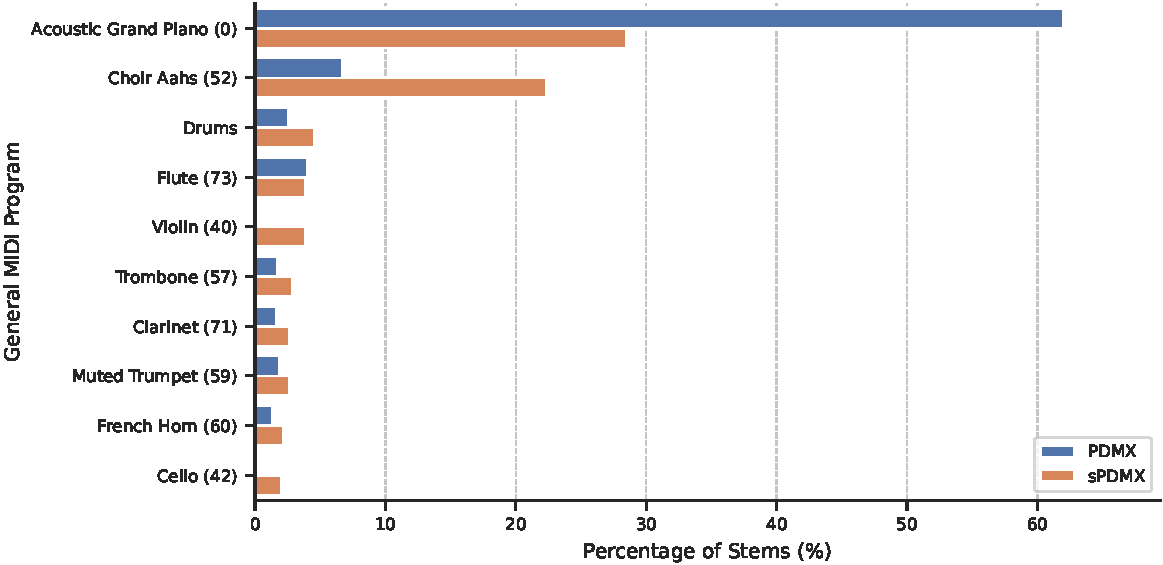
\includegraphics[width=\linewidth]{figures/gm_program_counts_compare.pdf}}
  \caption{Top-10 General MIDI programs by sPDMX (register-corrected) stem count (\texttt{all\_valid}; non-empty tracks), compared to raw PDMX MIDI \texttt{program\_change} shares.
  Shares are percentages within each inventory; the long tail outside these programs is omitted.
  After correction, mass concentrates in piano, choir/voice, drums, and common orchestral programs, motivating per-category Slakh and SA3 realify tuning on those families.}
  \label{fig:gm_programs}
\end{figure}

\section{Related work}
\label{sec:prior}

\textbf{Symbolic and stem datasets.}
Lakh MIDI~\cite{raffel2015large,raffel2016learning} established large-scale symbolic music as a research substrate.
PDMX~\cite{long2024pdmx,xu2024generating} emphasizes public-domain provenance at scale.
On the audio side, MedleyDB~\cite{bittner2014medleydb} and MUSDB18~\cite{rafii2019musdb18} provide recorded multitracks; Slakh2100~\cite{manilow2019cutting} synthesizes stems from MIDI with commercial libraries.
sPDMX targets Slakh-like stem structure from open symbolic data and redistributable soundfonts.

\textbf{Neural MIDI-to-audio.}
DDSP~\cite{engel2020ddsp} enables differentiable synthesis; MIDI-DDSP~\cite{wu2022midi} (trained on URMP~\cite{li2018creating}) and DDSP-Piano~\cite{renault2022diffpiano,renault2023ddsp_piano} (MAESTRO~\cite{hawthorne2018enabling}) provide neural stems for selected instruments.
We treat these as optional render paths within a broader factorial design rather than a single end-to-end synthesizer.

\textbf{Generative audio and evaluation.}
Stable Audio Open~\cite{evans2024stable} is our downstream training target; SA3~\cite{evans2026stable} supplies audio-to-audio realify.
Subjective evaluation uses a custom dual-scale web listening interface (content and realism, 0--100), with a labeled open reference and shuffled unlabeled conditions per excerpt.

\section{Method}
\label{sec:method}

\subsection{Pipeline overview}
\label{ssec:pipeline}

Given a PDMX song, we (1)~correct per-track General MIDI (GM) program IDs using track-name aliases (GM register), (2)~render each track to a mono stem, (3)~optionally apply SA3 realify conditioned on a caption and category-specific diffusion presets, and (4)~form a mixture by summing loudness-normalized stems with a uniform anti-clip gain (Slakh-style), targeting $-23$~LUFS~\cite{series2011algorithms}.

\subsection{Render families}
\label{ssec:render}

We define four render families before the realify factor:

\begin{itemize}
\item \textbf{Basic (A):} FluidSynth with a single default GM soundfont (SGM).
\item \textbf{Slakh (B):} Per listening category, a shortlist of soundfonts and an FX profile (\texttt{dry}/\texttt{light}/\texttt{warm}). At render time, one font is sampled per (song, category) from a seeded RNG, approximating Slakh-style timbral variety without closed VSTs.
\item \textbf{DDSP-basic (CA) / DDSP-Slakh (CB):} Route eligible piano and monophonic orchestral programs through DDSP-Piano / MIDI-DDSP; remaining tracks copy the corresponding basic or Slakh soundfont stems.
\end{itemize}

Crossing each family with optional SA3 realify yields eight ablation conditions (Table~\ref{tab:ablations}).

\begin{table}[t]
\centering
\caption{Factorial ablation conditions (render family $\times$ realify).}
\label{tab:ablations}
\vspace{1mm}
\small
\begin{tabular}{@{}lcc@{}}
\toprule
 & -- & SA3 \\
\midrule
Basic       & A1  & A2  \\
Slakh       & B1  & B2  \\
DDSP-basic  & CA1 & CA2 \\
DDSP-Slakh  & CB1 & CB2 \\
\bottomrule
\end{tabular}
\end{table}

\subsection{Per-category tuning listening}
\label{ssec:tuning}

Production Slakh and SA3 settings are not chosen globally.
Fig.~\ref{fig:gm_programs} shows that PDMX is filled with piano, choir/voice, and common orchestral programs; we therefore concentrate listening-tuned soundfont shortlists and SA3 realify presets on those high-mass categories (plus drums and other classes needed for full-song coverage), rather than spreading equal effort across the long GM tail.

On a fixed probe set of 24 stems (3 per category across piano, drums, strings, wind, voice, mallet, organ, and related classes), we ran blinded listening tests with randomized labels.
Listeners rated each variant on two 1--5 scales: \emph{content} (melody/rhythm/timing vs.\ a basic reference) and \emph{realism} (appropriate instrument timbre).

For Slakh patches, phases compared candidate soundfont banks and then FX profiles; aggregation selected per-category shortlists and FX, then locked production config.
For SA3 presets, phased sweeps over \texttt{init\_noise\_level}, prompt variant, and diffusion hyperparameters produced per-category winners; categories for which realify harmed quality (e.g., mallet, organ) disable realify in production.
Locked configs define the engineered A2/B1/B2 (and DDSP variants) used in the formal ablation study.

\section{Listening study: ablation}
\label{sec:listening}

We conducted a formal dual-scale listening study over all eight conditions in Table~\ref{tab:ablations}.
The open reference was A1 (basic); the same signal also appeared as a hidden reference among the shuffled unlabeled conditions when present.
Each trial presented a $\sim$10\,s stem excerpt on a single page: listeners rated every unique condition on both \emph{content adherence} and \emph{realism} (0--100).
Donor-copy DDSP fallbacks identical to their soundfont donors were omitted from the page and assigned the donor scores at aggregation.
The trial set comprised 2 stems $\times$ 10 listening categories (piano, drums, strings, wind, voice, mallet, organ, guitar, brass, polyphonic), for 20 rating pages.
We collected responses from $N{=}\textit{[TBD]}$ listeners.

\subsection{Results}
\label{ssec:mushra_results}

Table~\ref{tab:mushra} summarizes mean scores (\textit{placeholder}).
% TODO: replace with aggregate.py output.
Overall, condition \textbf{[TBD, e.g.\ B2]} achieved the best trade-off between content and realism and was selected as the production recipe for full-scale sPDMX.
Per-category breakdowns (not shown for space) informed remaining realify bypasses and shortlist adjustments.

\begin{table}[t]
\centering
\caption{Ablation listening means (0--100). \textit{Placeholder---replace after aggregation.}}
\label{tab:mushra}
\vspace{1mm}
\small
\begin{tabular}{@{}lcc@{}}
\toprule
Condition & Content $\uparrow$ & Realism $\uparrow$ \\
\midrule
A1  & -- & -- \\
A2  & -- & -- \\
B1  & -- & -- \\
B2  & -- & -- \\
CA1 & -- & -- \\
CA2 & -- & -- \\
CB1 & -- & -- \\
CB2 & -- & -- \\
\bottomrule
\end{tabular}
\end{table}

\section{Engineered sPDMX}
\label{sec:engineered}

Using the listening-selected recipe and the locked per-category Slakh/SA3 configs from Section~\ref{ssec:tuning}, we rendered the full PDMX-derived release set.
Each song directory contains mono stems and a loudness-normalized mixture~\cite{series2011algorithms}.
Metadata from PDMX (paths, instrumentation, durations) is retained alongside stem inventories so that models can train on stems, mixtures, or both.
Where neural DDSP coverage is incomplete, soundfont fallbacks preserve full song completeness.
Vocal stems use the soundfont (+ optional realify) path; lyric-conditioned singing-voice synthesis was left out of scope due to open-weight provenance constraints.

\section{Experiments: SAO on Slakh vs.\ sPDMX}
\label{sec:experiments}

To test whether listening-tuned large-scale stems improve generative modeling, we trained Stable Audio Open~\cite{evans2024stable} from scratch under matched budgets on (i)~Slakh2100~\cite{manilow2019cutting} and (ii)~sPDMX rendered with the Section~\ref{sec:listening} winner.
Both models generated audio for a fixed set of held-out text prompts.
In a second listening test, participants rated pairs of generations on content relevance to the prompt and perceived audio realism, and indicated overall preference.

\subsection{Results}
\label{ssec:sao_results}

Table~\ref{tab:sao} reports preference and scale means (\textit{placeholder}).
Listeners preferred sPDMX-trained SAO in \textit{[TBD]}\% of trials; content and realism scores were \textit{[TBD]} vs.\ \textit{[TBD]} (Slakh) and \textit{[TBD]} vs.\ \textit{[TBD]} (sPDMX).

\begin{table}[t]
\centering
\caption{SAO listening results. \textit{Placeholder---replace after Test~2.}}
\label{tab:sao}
\vspace{1mm}
\small
\begin{tabular}{@{}lccc@{}}
\toprule
Training data & Pref.\ \% $\uparrow$ & Content $\uparrow$ & Realism $\uparrow$ \\
\midrule
Slakh2100 & -- & -- & -- \\
sPDMX (winner) & -- & -- & -- \\
\bottomrule
\end{tabular}
\end{table}

\section{Conclusion}
\label{sec:conclusion}

We presented sPDMX, a listening-tuned pipeline that turns PDMX into multi-stem audio via Slakh-style soundfont variety, optional DDSP, and SA3 realify.
Ablation listening guided the production recipe; training SAO on sPDMX versus Slakh2100 tested downstream value of that recipe.
Future work includes broader listener pools, automatic content-fidelity gates, and releasing configs alongside the dataset for reproducible regeneration.

% Provenance note (brief): FluidSynth soundfonts; MIDI-DDSP/URMP; DDSP-Piano/MAESTRO; SA3 licensed weights.

\vfill\pagebreak

\section{REFERENCES}
\label{sec:refs}
\bibliographystyle{IEEEbib}
\bibliography{main}

\end{document}
